%%%%%%%%%%%%%%%%%%%%%%%%%%%%%%%%%%%%%%%%%%%%%%%%%%%%%%%%%%%%%%%%%%%%%%%%%%%%%
\section{SSCAIT: Student StarCraft\\ AI Tournament}\label{subsecSSCAIT}

The Student StarCraft AI Tournament (SSCAIT) is the StarCraft AI competition with the highest number of total participants. There are three fundamental differences between SSCAIT and the remaining two competitions:
\begin{enumerate}
  \item SSCAIT is an online-only event. Unlike AIIDE or CIG, it is not co-located with a scientific conference / event. \item There are two phases of SSCAIT each year: a~competitive {\em tournament phase}, lasting for up to four weeks and a {\em ladder phase} which runs for the rest each year. In other words, SSCAIT is live at all times with only a few short interruptions for maintenance.
  \item Games are played one at a time and are publicly streamed live on Twitch.tv.\footnote{http://www.twitch.tv/sscait} and SmashCast.tv. The AIIDE and CIG competitions instead play as many games as possible at maximum speed, with no broadcast.
\end{enumerate}

SSCAIT's {\em tournament phase} takes place every winter in late December and early January. 
%At the time of writing of this paper, SSCAIT 2017/18 tournament was in progress with 78 participants. Since the 2017/18 results are still incomplete, we cover the results of previous SSCAIT year.

\begin{figure}[t]
  \centering
  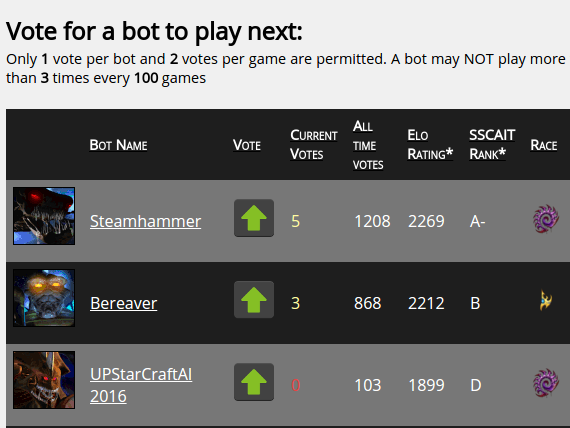
\includegraphics[width=1\columnwidth]{fig/sscait-voting.png}
  \caption{A web-based interface allowing SSCAIT viewers and bot programmers to vote for the next ladder match.}
  \label{figSSCAITvoting}
\end{figure}

%%%%%%%%%%%%%%%%%%%%%%%%%%%%%%%%%%%%%%%%%%%%%%%%%%%%%%%%%%%%%%%%%%%%%%%%%%%%%
\subsection{SSCAIT History}

The first SSCAIT was organized in 2011 by Michal \v{C}ertick\'{y}, as a part of the ``Fundamentals of Artificial Intelligence'' course at Comenius University in Bratislava, Slovakia. It started as a closed event, with 50 local students competing for extra points for their course evaluation. Since the event received a lot of positive feedback from the participants, the organizers decided to open it for the international public and for non-students next year~(although the word ``Student'' remained in the competition name for historic reasons). 

SSCAIT changed significantly over the course of 2012 -- both in terms of the format and technology behind it. The organizers implemented a collection of simple Python and AHK scripts that were able to run and evaluate the bot games automatically. This allowed for the creation of 24/7 bot {\em ladder} with online live stream, similar to the one available today.\footnote{The SSCAIT bot ladder was inspired by an older automated StarCraft bot ladder, available at that time at http://bots-stats.krasi0.com/} The live-streamed ladder simplifies the bot debugging process~(since bot authors can watch their creations play all kinds of AI opponents), encourages continuous development over the whole year and accelerates the growth of StarCraft AI research community. 

The registration of new bots on the ladder was simplified in 2013 with the introduction of web-based user interface for bot creators. They can now upload new versions of their bots to the ladder at any time. In 2014, the custom automation scripts were replaced by Tournament Manager Software, developed originaly for AIIDE competition (details in section~\ref{secTournamentManagerSoftware}), which needed to be heavily modified in order to work with SSCAIT user and game databases and to support the ladder format. Further modifications and the introduction of Dockerized multi-platform version of StarCraft~\cite{maly2018multi} are planned soon. 

Currently, SSCAIT is organized by the {\em Games \& Simulations} Research Group\footnote{http://gas.fel.cvut.cz/} -- part of Artificial Intelligence Center at Czech Technical University in Prague.

%%%%%%%%%%%%%%%%%%%%%%%%%%%%%%%%%%%%%%%%%%%%%%%%%%%%%%%%%%%%%%%%%%%%%%%%%%%%%
\subsection{SSCAIT 2017/18 Tournament \& Ladder}\label{subsecSSCAITnews}

\begin{figure}[t]
  \centering
  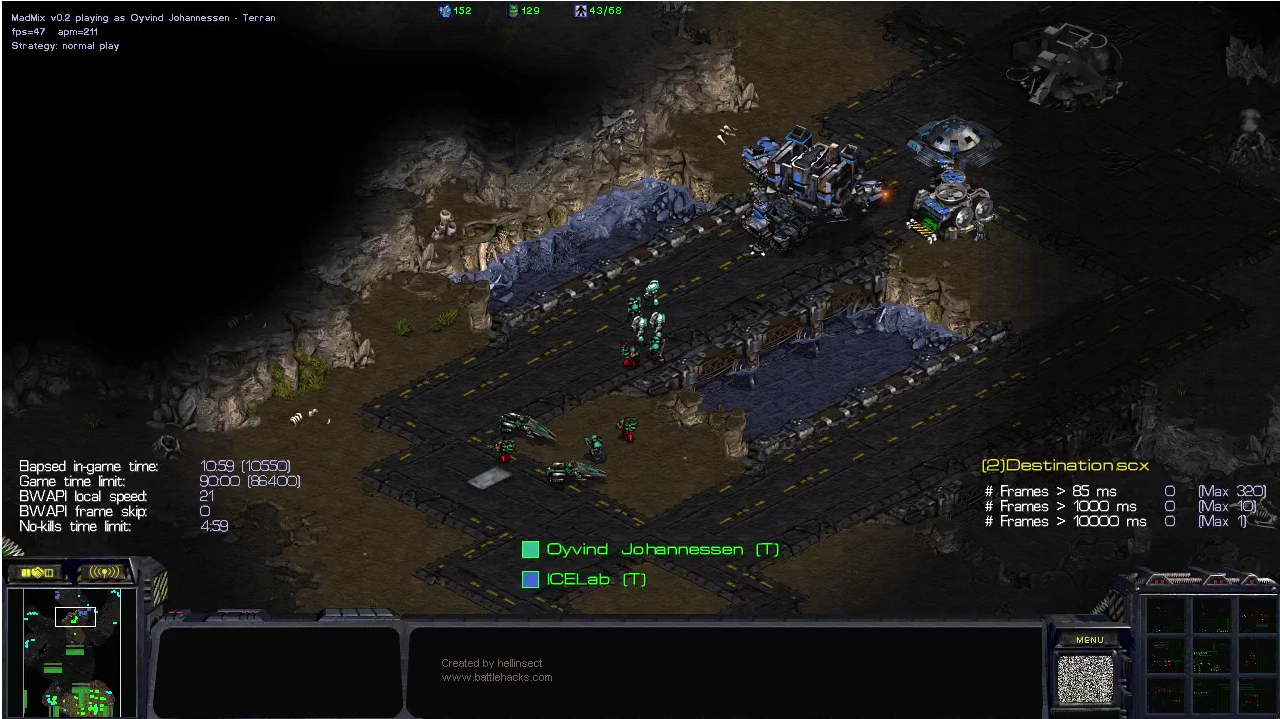
\includegraphics[width=1\columnwidth]{fig/sscait-stream.png}
  \caption{SSCAIT live stream running in HD resolution and controlled by the custom observer script~\cite{mattsson2015automatic}.}
  \label{figSSCAITstream}
\end{figure}

The activity of bot programmers and the general public surrounding SSCAIT has grown considerably over the course of the past year, with new members to the organizing team making a number of improvements to the live stream, and better community engagement during the Ladder phase.

First, the ladder phase was updated, with SSCAIT introducing so-called ``weekly reports''. Every weekend, there is a 1-2 hour long segment of curated AI vs. AI matches with insightful commentary on the live stream. Second, a voting system was implemented, allowing bot programmers and viewers to select which bots will play the next ladder match on live stream (Figure \ref{figSSCAITvoting}). This not only supports viewer engagement, but also greatly simplifies bot debugging process. Bot programmers can now quickly test their newest updates against specific opponents. This change might have contributed to the significant increase in bot update frequency. Approximately 5-6 bots are updated every day, in contrast to 0-2 updates per week in 2015.

Another update was the introduction of ``minitournaments'' to SSCAIT. These are easily configurable, irregular and unofficial short competitions, taking up to one day. The format of these minitournaments and the selection of participants is usually up to the stream viewers and moderators. Visual quality of the stream was improved by updating the custom observer script~\cite{mattsson2015automatic} which now moves the camera fluently to the most interesting parts of the game in real time and displays SSCAIT-related information on top of the game. The stream was also upgraded to HD using a ``resolution hack'' (Figure \ref{figSSCAITstream}). 
The overall number of stream views has increased to 376,920 views on Twitch.tv and additional 434,216 views on SmashCast.tv over the past 12 months. Two additional metrics were added to the ladder ranking system due to popular demand: ELO rating~\cite{elo1978rating}, which is used in adversarial games like chess, and ``SSCAIT rank'', based on so-called ``ICCUP ranking system'', typical for competitive StarCraft.

\subsubsection*{SSCAIT Tournament Phase Updates}

The 2017/18 installment of SSCAIT's tournament phase took place during four weeks at the end of December 2017 and beginning of January 2018 and sported 78 participants. The tournament was divided into two divisions:

\emph{Student Division}: Round Robin tournament of 6006 games, where every bot played two games against every opponent. Only the bots created by individual students were considered ``student'' bots and were eligible for victory in this division. Other bots were tagged as ``mixed-division'' bots (they played the games, but could not win the student division title). Winners of the student division in 2017/18 were:
  \begin{enumerate}
	\item Wulibot, University of Southern California (USA) with 124 wins
	\item LetaBot (Martin Rooijackers), University of Maastricht (Netherlands) with 109 wins
	\item Carsten Nielsen, Technical University of Denmark (Denmark) with 101 wins
  \end{enumerate}
The student division of SSCAIT exists so that the students stand a chance of winning in the presence of more experienced, non-student participants and team-created bots.

\emph{Mixed Division}: After the student division ended, sixteen bots with the most wins among all the participants were selected for the additional “mixed division” double elimination bracket, consisting of 30 matches (best of 3, 5, or 7 games), which can be seen in Figure \ref{figSSCAITbracket}. 

\begin{figure}[t] 
  \centering
  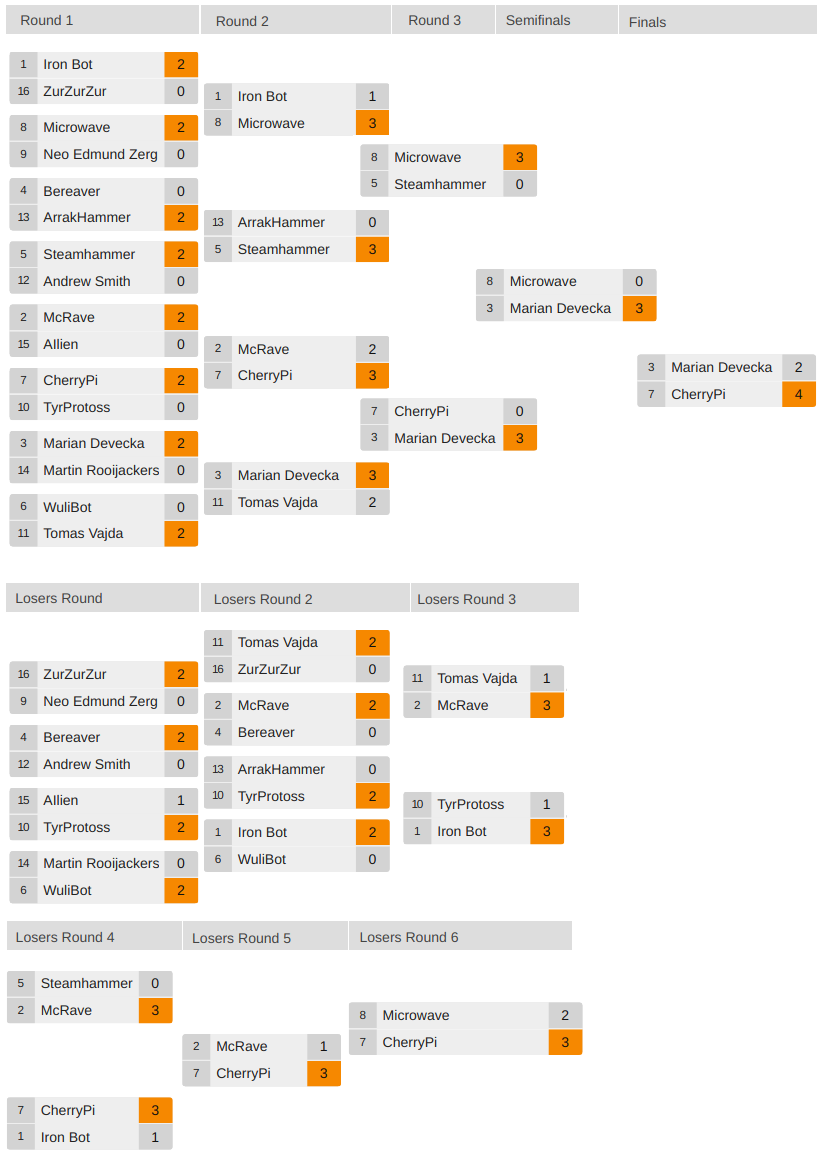
\includegraphics[width=1.04\columnwidth]{fig/sscait-bracket.png}
  \caption{SSCAIT 2017/18 mixed division double elimination bracket.}
  \label{figSSCAITbracket}
\end{figure}  

{\em CherryPi}, created by the Facebook AI Research team won the mixed division by beating KillerBot by Marian Devecka 4-2 in the finals. Interestingly, CherryPi encountered KillerBot earlier in the tournament (in winner's round 3) and lost that match 0-3, dropping down to the losers bracket. The bot then managed to win the whole losers bracket, meet Killerbot again in the finals and win by exploiting its experience from their previous games. More information about CherryPi can be found in Section~\ref{secBots}.
%{\em LetaBot} (created by Martin Rooijackers) won the mixed division elimination bracket in addition to winning the student division, after beating {\em Krasi0bot} (created by Krasimir Krystev) 3 to 1 in the finals~(fig. \ref{figSSCAITbracket}). {\em LetaBot} had hard-coded special strategies against specific opponents. It successfully executed an ``SCV rush'' in the final games -- a strategy for which {\em Krasi0bot} was not prepared. 
All the elimination bracket games were published as videos with commentary on SSCAIT YouTube channel\footnote{\url{https://goo.gl/icbYdK}} and as replay files on SSCAIT website.\footnote{\url{http://sscaitournament.com/index.php?action=2017}} 

% This is not relevant to the paper
%Tournament winner, Martin Rooijackers, has recently been invited to have a talk about this achievement at a business-oriented AI conference {\em World Summit AI}.\footnote{\url{http://worldsummit.ai/}} 



